\chapter{Anhang}
\section{Installation von Lejos in Eclipse}
In diesem Abschnitt soll beschrieben werden wie die Erweiterung \textbf{Lejos} in die Java IDE Eclipse installiert wird.\\ 
- Eingehen auf die Reihenfolge der Installationen\\
- Alternativer Weg zu meinem Installationsweg \\
\section{Testprogramm des Ultraschallsensors}
\begin{figure}[htb]
\centering
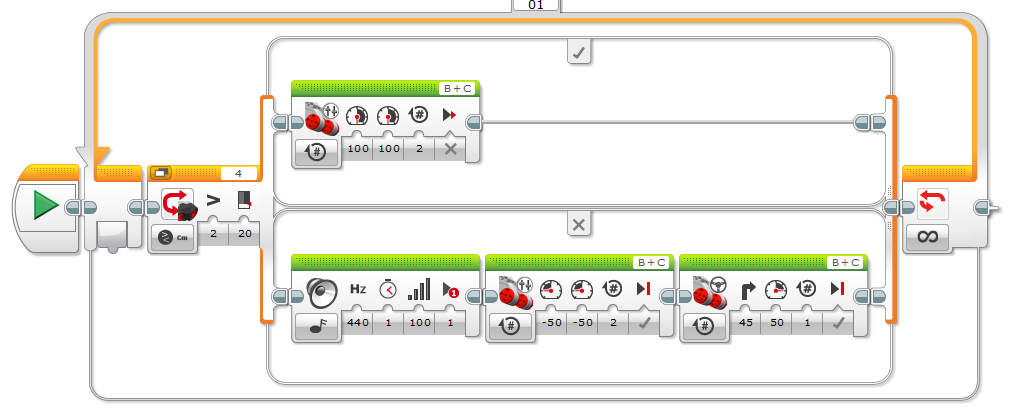
\includegraphics[width= 15cm]{Prog_Ultraschallsensor}
\caption{Lego-Programm zum Test und Kennenlernen des Ultraschallsensor}
\label{fig:ultraschallsensorprog}
\end{figure}
Im der Abbildung \vref{fig:ultraschallsensorprog} wird das, mit der Lego-Programmierumgebung erstellte, Programm dargestellt.\\
Das Programm besteht aus zwei ineinander geschachtelte Schleifen. Die äußere Schleife besitzt keine Abbruchbedingung. Die innere der beiden Schleifen überwacht den Ultraschallsensor und entscheidet je nach Ergebnis des Sensors, was der Roboter machen soll.\\
Trifft der Vergleich \textbf{Vergleich erläutern} zu so fährt der Roboter mit Höchstgeschwindigkeit nach vorne, solange bis sich jedes der Räder genau zweimal gedreht hat. Danach wird auf Grund der Endlosschleife wieder der Ultraschallsensor abgefragt. Diesen Zweig erkennt man an dem Haken über den Anweisungen.

Trifft der Vergleich nicht zu, wird zuerst ein Ton über den integrierten Lautsprecher ausgegeben. Dieser Ton ist ein 440Hz Ton und wird mit voller Lautstärke eine Sekunde lang ausgegeben. Anschliesend fährt der Roboter mit halber Kraft zwei Radumdrehung zurück. Ist dies erledigt, soll sich der Roboter um 45 Grad drehen. Aufgrund der Endlosschleife wird wieder von Vorne begonnen und der Ultraschallsensor wird abgefragt. Dieser Zweig ist in der Darstellung \vref{fig:ultraschallsensorprog} an dem darüber stehenden x zuerkennen.

\section{Testprogramm des Lego-Farbsensor}
\begin{figure}[htb]
\centering
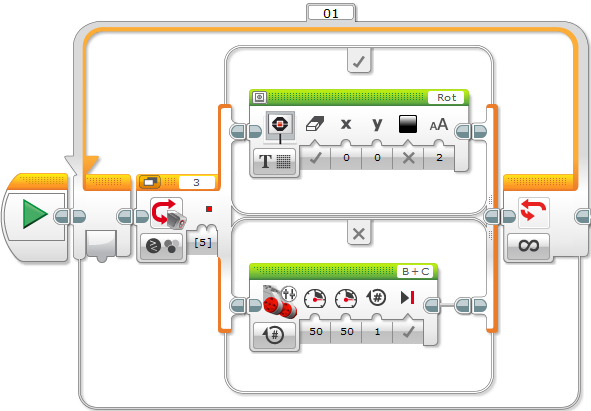
\includegraphics[width= 14cm]{Prog_LichtsensorLego_v1}
\caption{Lego-Programm zum Test und Kennenlernen des Farbsensors von Lego}
\label{fig:farbsensorprog}
\end{figure}
Das unter Abblidung\vref{fig:farbsensorprog} dargestellte Programm, ist ein Beispielprogramm für den Lego eigenen Farbsensor. 
Mit Hilfe dieses Programms wurde festgestellt, dass der Sensor manche Farben fehlerhaft erkennt. Dies ist zurückzuführen auf seine niedrige Farbauflösung. Diese Detektiert lediglich acht verschiedene Farben.
\section{Installation Vision subsystem V4}
Aufgrund der schlechten Farbauflösung des Lego eigenen Sensors, wurde ein weiterer Sensor angeschafft. Für diesen Sensor mussten weiter Vorarbeiten und Änderungen vorgenommen werden.
\paragraph{Besonderheiten dieses Sensors}
-Reaktion auf der Kamera auf fluoreszierendes Licht!!!

\paragraph{Installation der Kamera-Gerätetreiber unter Windows7}
Die Kamera wurde mittels USB-A auf Micro-USB Kabel mit dem PC verbunden.
Die Treiber wurden von der Seite \url{http://mindsensors.com/index.php?module=pagemaster&PAGE_user_op=view_page&PAGE_id=78} geladen.\\
Mit diesen Treibern kann anschließend das Programm NTXCamView ausgeführt werden. Dieses Programm kann unter \url{http://nxtcamview.sourceforge.net/} geladen werden.\\
Mit Hilfe dieses Programms kann die Kamera Bilder erstellen und die Farbe für die Detektion festgelegt werden. 

Besonderheit dieser Treiberinstallation ist, dass die Treiber per Hand geladen werden müssen und nicht automatisch geladen werden.

\textbf{Deutsche Anleitung zum Installieren hinzufügen!!!}
Für die Installation ist eine Internetverbindung notwendig. Es wird explizit angegeben an welchen Stellen diese benötigt wird. Für eine spätere Nutzung ist keine Internetverbindung vorgesehen.
\begin{enumerate}
\item Download der Geräte Treiber \textbf{Internetverbindung notwendig}
\item Download des Programms NTXCamView \textbf{Internetverbindung notwendig}
\item bla bla 
\end{enumerate}

